\documentclass{article}
\usepackage[utf8]{inputenc}
\usepackage[T1]{fontenc}
\usepackage{graphicx}
\usepackage{hyperref}
\usepackage{geometry}
\geometry{margin=1in}

\title{HELLESPONTS}
\date{Encyclopaedia Britannica (1771)}

\begin{document}
\maketitle

\section*{Historical source}
\textbf{Entry ID:} \texttt{entry-hellesponts-1017} \\
\textbf{Volume ID:} 144850367 \\
\textbf{Character Count:} 871

\subsection*{Extracted Text}
HELLESPONTS, the entrance of the flereights which divides Afa from Europe, and paths from the Archi- Vol. II. No. 59.

HEM pelago to Confantainople. It is now called the Darda- nelles, and is about two miles wide.

HELM \_g? a flip\_, is a piece of timber fallenred into the reader, which comes forward into the literary, or place where the prefix at the helm flere the flag, by holding the whiplaff in his hand, which is joined to the helm. They begin however to be left off, fleeting- which being died in their room.

There are several terms in the tea-language relating to the helm; as, \_hear up the helm;\_ that is, let the flip my or most large before the wind. \_Helm amid fribp\_ or \_right the helm;\_ that is, keep it even with the middle of the hip. \_Part, the helm\_, put it over the the of field of the hip. \_Starkbard the helm\_, put it on the right side of the flip.



\section*{Source record}
\begin{itemize}
\item \textbf{Dataset:} \texttt{NationalLibraryOfScotland/encyclopaedia\_britannica\_illustrated}
\item \textbf{Dataset Revision:} \texttt{309f765b1ecc83e0a7f7762e44b4a927a7555443}
\item \textbf{Page ID:} \texttt{britannica:309f765b1ecc83e0a7f7762e44b4a927a7555443:train:1017} \\
  \textbf{Filename:} \texttt{page-1017-5395deb0e141.jpg} \\
  \textbf{Row Index:} 1017 \\
  \textbf{SHA256:} \texttt{5395deb0e1413694...}
\end{itemize}

\begin{figure}[h]
\centering
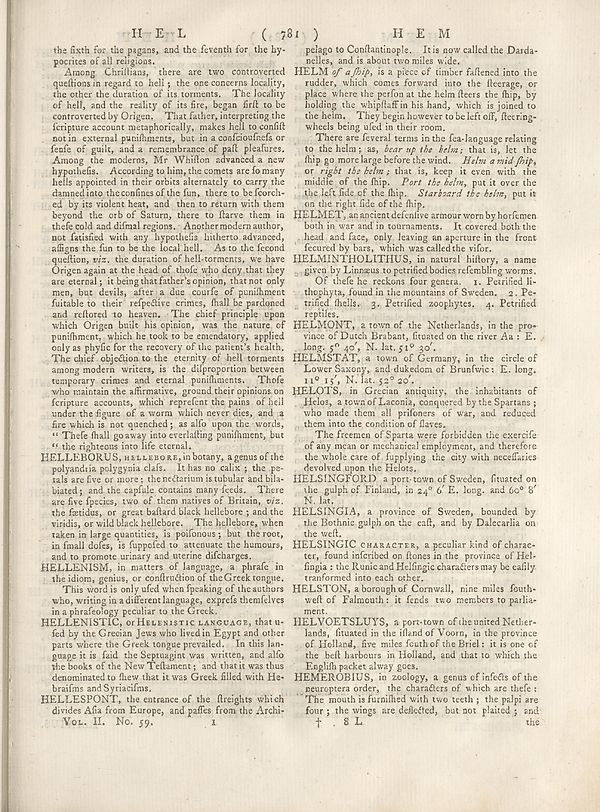
\includegraphics[width=0.85\textwidth]{../scans/page-1017-5395deb0e141.jpg}
\caption*{Source scan: \texttt{page-1017-5395deb0e141.jpg}}
\end{figure}

\end{document}
